\documentclass{article}


\usepackage[a4paper,top=1cm,bottom=1cm,left=1cm,right=1cm,marginparwidth=
1cm]{geometry}


\usepackage{multicol}
\PassOptionsToPackage{hyphens}{url}\usepackage{hyperref}

\usepackage{titlesec}

\titlespacing\section{0pt}{12pt plus 4pt minus 2pt}{0pt plus 2pt minus 2pt}
\titlespacing\subsection{0pt}{12pt plus 4pt minus 2pt}{0pt plus 2pt minus 2pt}
\titlespacing\subsubsection{0pt}{12pt plus 4pt minus 2pt}{0pt plus 2pt minus 2pt}


\usepackage{graphicx}
\usepackage[font=small,skip=4pt]{caption}
\graphicspath{ {.} }

\pagenumbering{gobble}

\title{The challenge of running Python on the Arduino}
\author{Christian Krause \small(christian.k@netcom-mail.de)\\[0.1cm]{\small Supervisor: Helmut Ruf}}
\date{\small Student Research Center Ochsenhausen-Germany}

\usepackage{etoolbox}
\makeatletter
\patchcmd{\@maketitle}{\null\vskip 2em}{}{}{}
\makeatother

\begin{document}
\maketitle
\begin{multicols}{2}
\section{Programming on the Arduino}
\noindent The Arduino is a very popular microcontroller that is often used to teach the basics of programming at schools. The programming language used for the Arduino is almost always C, which is a compiled low-level programming language. This means that it is very fast and has low memory demand. The drawback is, C is more difficult to learn than higher-level programming languages like Python. The difference between high- and low-level programming languages is the level of control the user has over the system. This can be an advantage for performance-critical applications, but high-level programming languages are generally easier to learn.% For example in Python, it is very easy to create a List and to insert or remove values. When attempting this in C, you quickly encounter pointers and other low-level concepts that can be very difficult for beginners.

\section{The Challenge}
\noindent This raises the question why Python is not used to teach programming on the Arduino. The problem is, that the Arduino Uno only has 2 kB of RAM and 32 kB of program memory \cite{Q1}. The Python interpreter alone requires over 30 mB of memory, not to mention its dependency on a large standard library. Running a Python executable requires a much faster CPU and orders of magnitude more RAM than the Arduino UNO has to offer. %So, at first glance, running Python on an Arduino seems impossible. But there is a project that attempts to solve this problem; MicroPython is an implementation of Python for microcontrollers, designed to use as few resources as possible. MicroPython is able to run a minimal subset of python with as little as 256 kb of flash and  16 kb of ram. But the Arduino Uno still only has an eigth of the capacity required to run MicroPython. 
The reason Python demands more resources compared to C lies in their respective workings. To run a .c file, the C compiler translates it into machine code, which can then be executed. A python file on the other hand is run by the Python interpreter, which runs a Python file line by line. This is a lot slower than a compiled C executable, but it enables a lot of the abstractions which make Python an easier, higher-level language than C.

\section{The solution: Pyduino}
\noindent My project, called Pyduino, aims at unifying the easy syntax of Python with the speed of C to run Python-like programs on the Arduino microcontroller. To achieve this, I developed a new programming language, Pyduino. The syntax of Pyduino is heavily inspired by Python \cite{Q2}. \\
An important feature of Pyduino is, that the same code can run on the PC and the Arduino. This feature is particularly helpful when quickly testing a program. Instead of waiting for it to be uploaded to the Arduino, which can take serveral seconds, you can simply run it on the PC.
Running the same code on multiple platforms that are very different, like a PC and an Arduino comes with some challenges. For example printing output to a console is only possible on the PC, while the Arduino has the ability to connect to actuators and sensors via its I/O pins.
Pyduino solves this problem by utilizing the serial connection between the Arduino and the PC. If you program an Arduino conventionally using C, any output that needs to be visible to the user is sent to the PC through this connection.
 In Pyduino programs, this bidirectional connection is not only used for output, but also for advanced features like function calls. If there is a program running on the PC that needs to use the I/O pins of the Arduino, for example to turn on an LED or to read from a sensor, it sends a request to the Arduino using a serial protocol that I developed. The Arduino then executes this request and sends the result back to the PC. This connection can also be used for custom function calls between the Arduino and the PC. Whenever a function is defined in Pyduino, the programmer has the option to specify where it is executed. 
 For instance, if the Arduino requires the result of a computationally intensive function, you can designate it to run on the PC by adding the @main decorator in front of the function. This instructs Pyduino to execute the function on the PC. When the Arduino needs this function executed, it sends a request to the PC, which then processes the function and returns the result to the Arduino\\
In some cases, this can lead to massive performance improvements. 
In this example, I used a recursive Fibonacci implementation to compute fib(40). When running this function solely on the Arduino, it takes about 18 minutes to complete. However, when the function is annotated with the @main decorator to execute on the PC, it finishes in about 440 ms when directly run on the PC, calling it from the Arduino takes 447 ms. If you implement the fibonacci function in C and run it on the PC, it takes 436 ms to complete, while the Python implementation took 18 seconds. This demonstrates that in certain scenarios, Pyduino approaches the speed of C and significantly outperforms Python. \\
\makebox[10pt][l]{%
\begin{minipage}{.5\textwidth}
\centering
    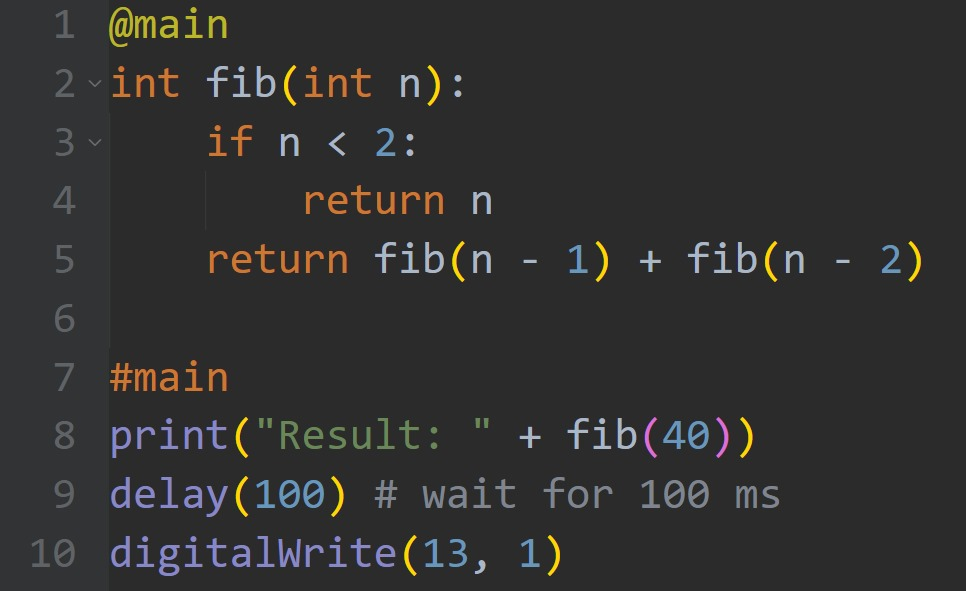
\includegraphics[width=6cm]{code}
 %\captionof{figure}{Pyduino example code}
\end{minipage}
}
\\\\
Additionally, I developed a VS Code extension for Pyduino to make it as easy as possible to write Pyduino code \cite{Q3}. The extension can be easily installed from the VS Code marketplace and it provides syntax highlighting and error detection for Pyduino files. A Pyduino file can be run by clicking the "Run Pyduino" button, the extension handles the compilation and execution of the code for both the PC and the Arduino seamlessly.
\section{Conclusion}
\noindent Overall, I developed Pyduino, a new programming language that is easy to learn but is still fast enough to run on the Arduino. Pyduino has many features that make it easy for beginners, including a VS Code plugin with syntax highlighting and error detection. This plugin is publicly available on the VS Code marketplace \cite{Q3}.


\begin{thebibliography}{99}
\bibitem{Q1} 
\url{https://docs.arduino.cc/hardware/uno-rev3/#tech-specs}
\bibitem{Q2}
\url{https://github.com/Bergschaf/Pyduino}
\bibitem{Q3}
\url{https://marketplace.visualstudio.com/items?itemName=Bergschaf.pyduino-extension}
\end{thebibliography}
\end{multicols}

\end{document}


